\documentclass[border=2pt]{standalone}
\usepackage{tikz}
\usetikzlibrary{arrows.meta,topaths}

\begin{document}
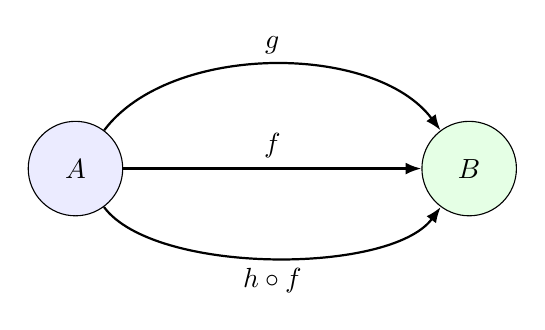
\begin{tikzpicture}[
  object/.style={draw,circle,minimum size=12mm,inner sep=1pt},
  morphism/.style={-{Latex[length=2mm]},thick}
]
  \node[object,fill=blue!8] (A) at (0,0) {$A$};
  \node[object,fill=green!10] (B) at (5,0) {$B$};

  \path[morphism]
    (A) edge node[above] {$f$} (B)
    (A) edge[controls={(1.2,1.6) and (3.8,1.6)}] node[above] {$g$} (B)
    (A) edge[out control={+(1,-1.35)},in control={+(-1,-1.35)}] node[below] {$h\circ f$} (B);
\end{tikzpicture}
\end{document}
